\subsubsection{Detalles de la actividad}
En esta actividad, se diseñó la interfaz del sistema en Figma, un software de diseño de interfaces de usuario. El diseño se realizó en base a los requerimientos recogidos en la actividad anterior, y se dividió en módulos para facilitar el desarrollo y la implementación. El prototipo final alcanzó un nivel de madurez muy alto, lo que permitirá una implementación ágil y eficiente en la siguiente fase del proyecto segun SCRUM.\\
\href{https://www.figma.com/proto/sV0jV2oSvDyUHLI0Pm1KzV/DPSEC?node-id=563-3455&t=SQIVi97HhkuWXdes-1&scaling=scale-down&content-scaling=fixed&page-id=0%3A1&starting-point-node-id=21%3A4&show-proto-sidebar=1}{Ver prototipo en Figma}

\begin{figure}[!htb] 
    \centering 
    \caption{Diseño de la interfaz de pagina principal publico} 
    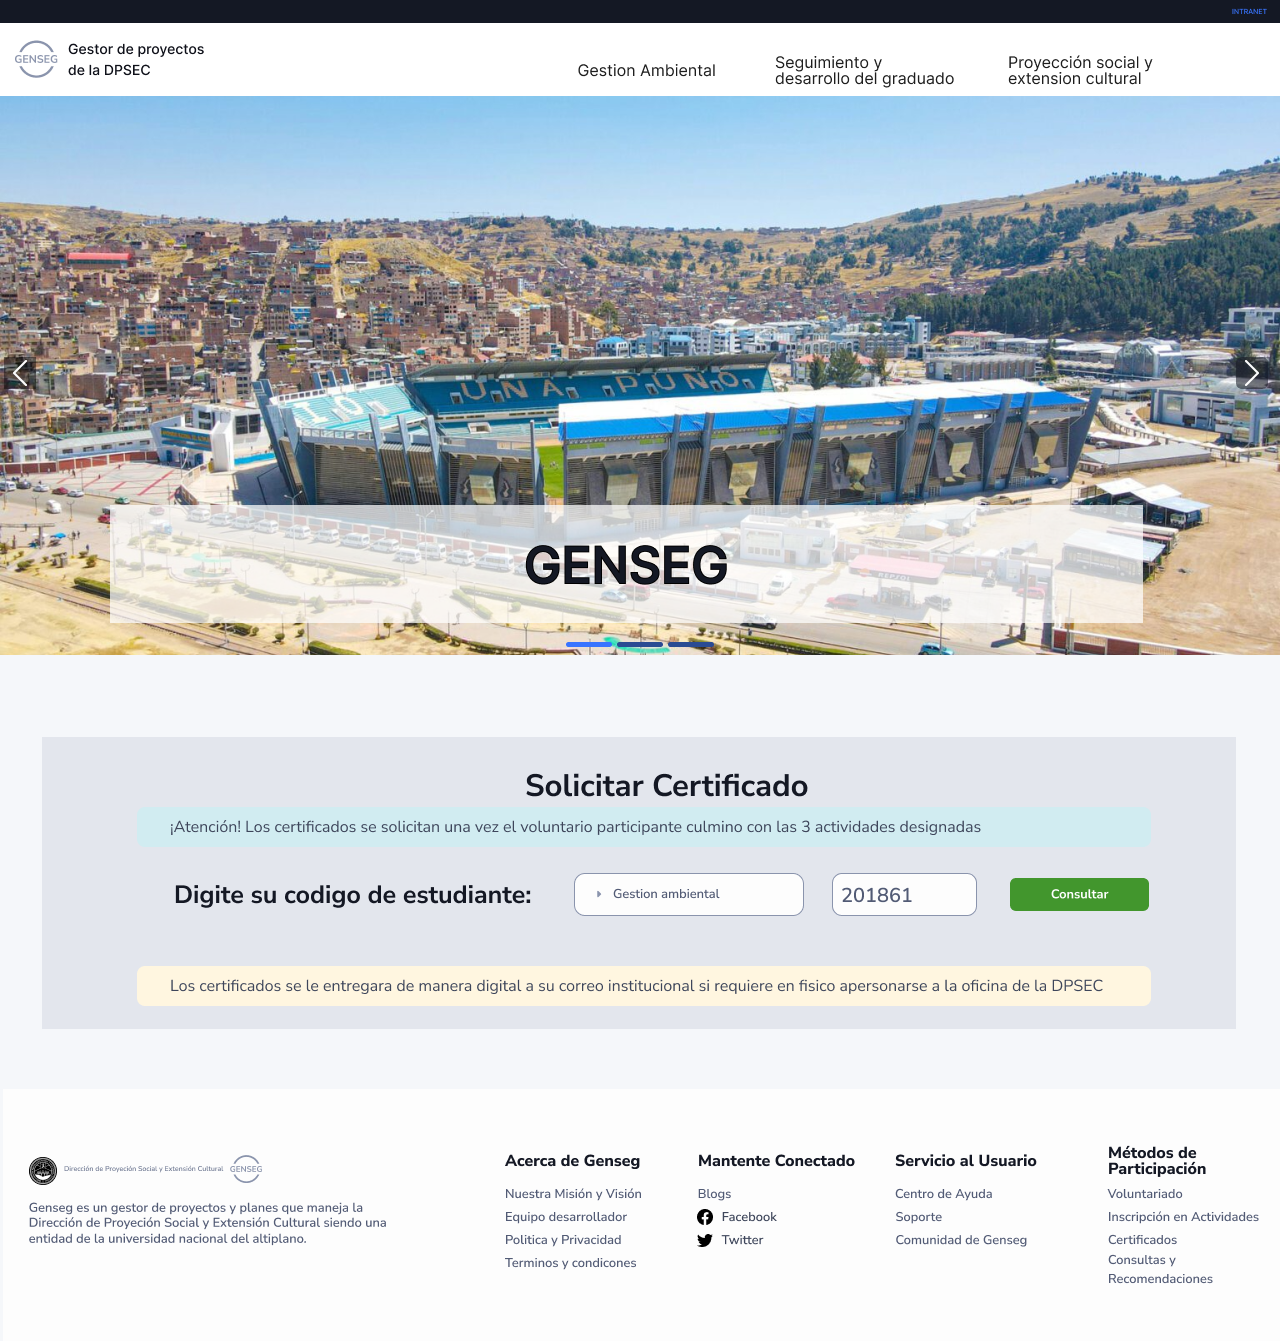
\includegraphics[width=0.8\textwidth]{images/paginaprincipal.png} 
    \label{fig:paginaprincipal} 
\end{figure} 
\FloatBarrier

\begin{figure}[!htb] 
    \centering 
    \caption{Diseño de solicitud de certificados} 
    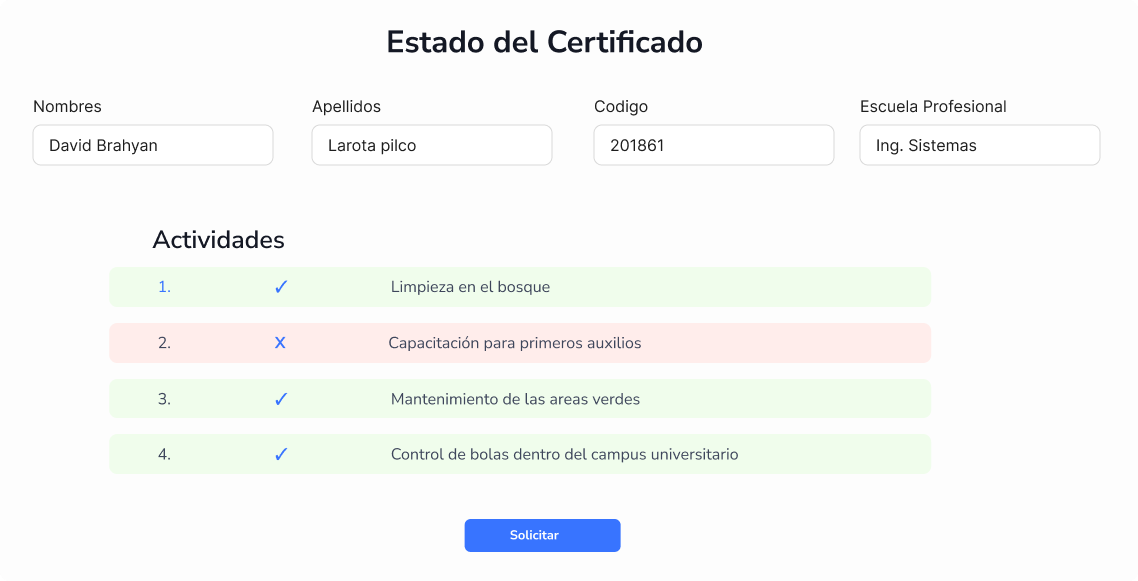
\includegraphics[width=0.8\textwidth]{images/certificado.png} 
    \label{fig:certificado} 
\end{figure} 
\FloatBarrier

\begin{figure}[!htb] 
    \centering 
    \caption{Intranet - Login} 
    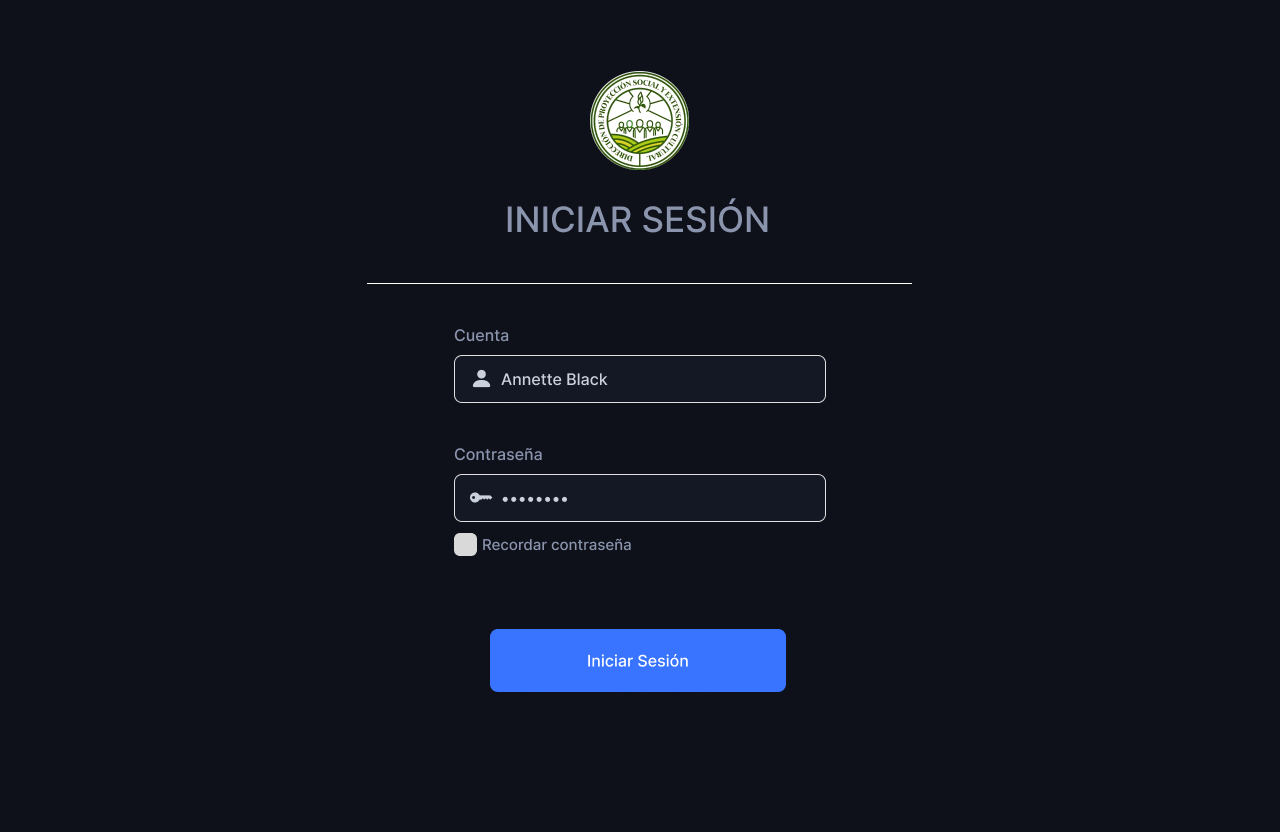
\includegraphics[width=0.8\textwidth]{images/intranet_login.png} 
    \label{fig:intranet_login} 
\end{figure} 
\FloatBarrier

\begin{figure}[!htb] 
    \centering 
    \caption{Intranet - Escoger roles} 
    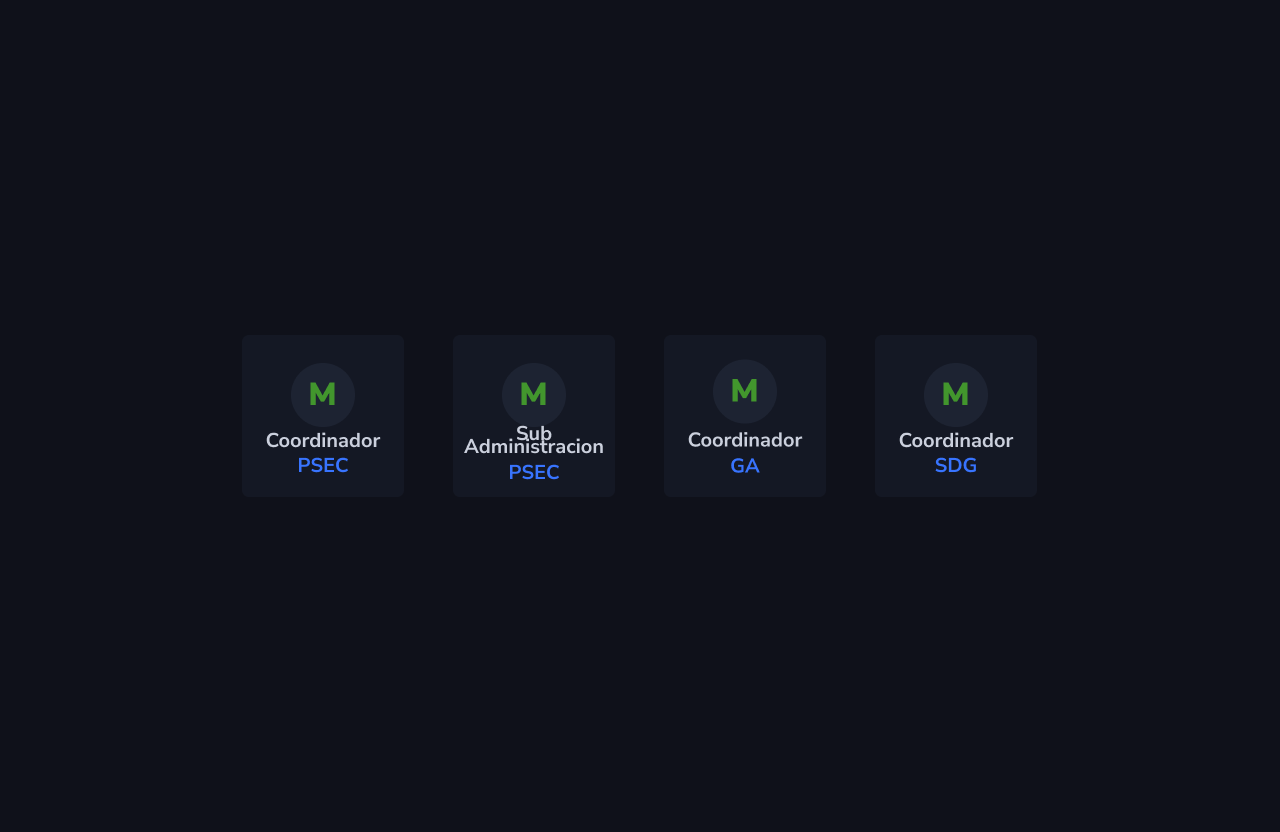
\includegraphics[width=0.8\textwidth]{images/roles.png} 
    \label{fig:roles} 
\end{figure} 
\FloatBarrier

\begin{figure}[!htb] 
    \centering 
    \caption{Intranet - Pagina principal} 
    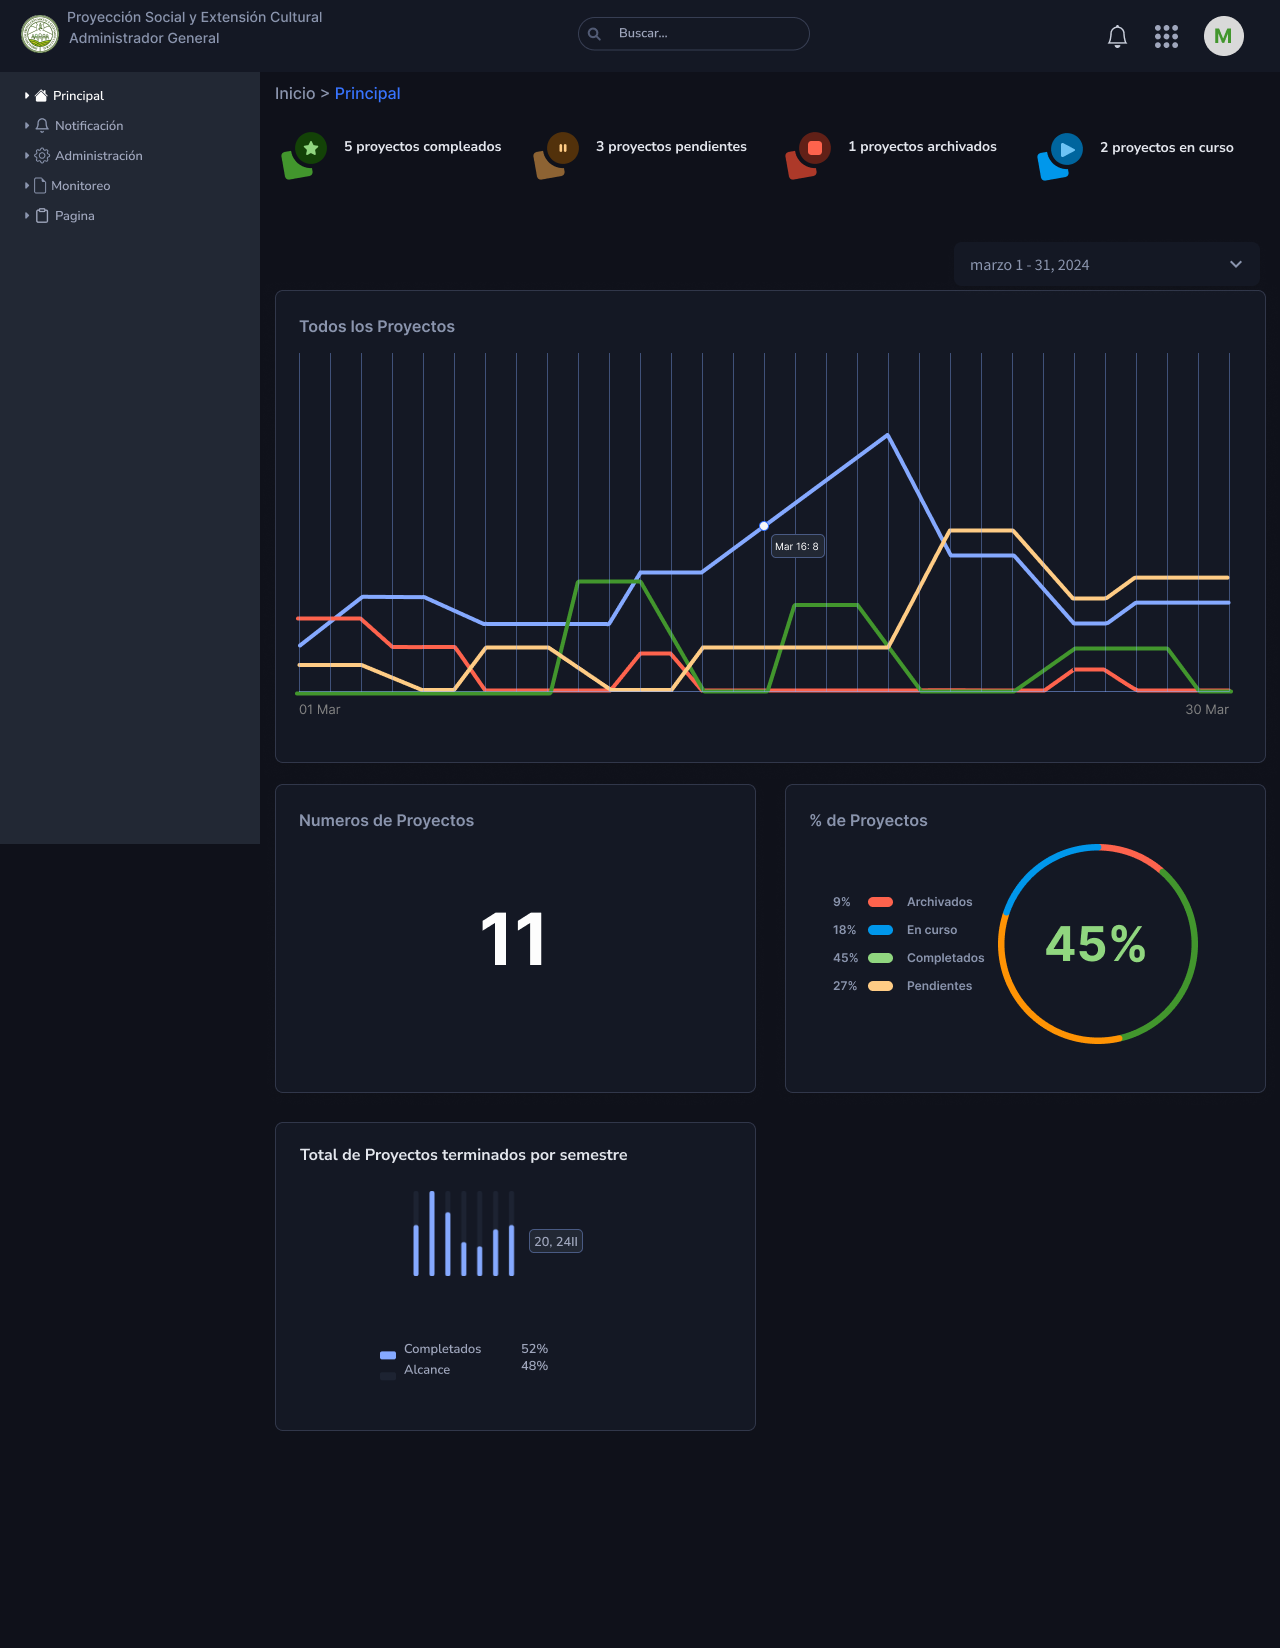
\includegraphics[width=0.8\textwidth]{images/principal.png} 
    \label{fig:principal} 
\end{figure} 
\FloatBarrier

\begin{figure}[!htb] 
    \centering 
    \caption{Intranet - Vista de Proyectos} 
    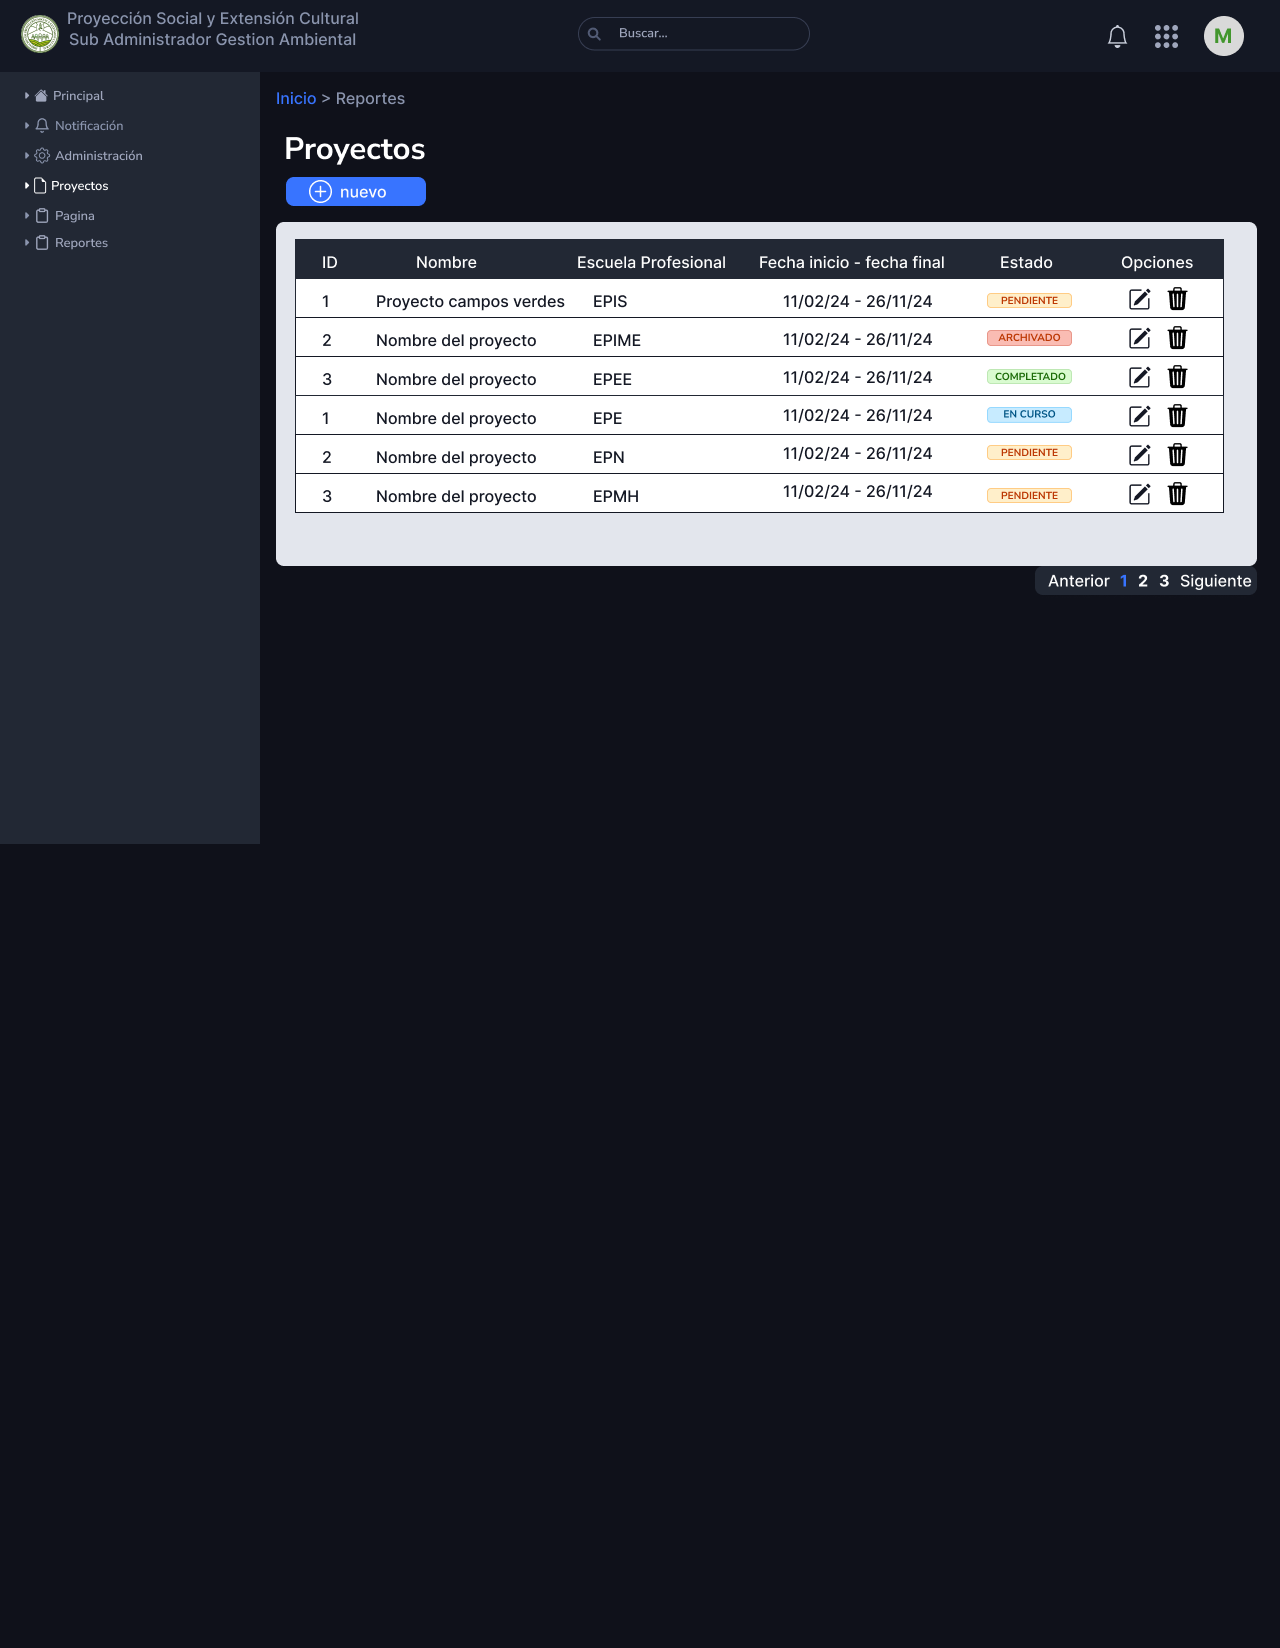
\includegraphics[width=0.8\textwidth]{images/proyectos.png} 
    \label{fig:proyectos} 
\end{figure} 
\FloatBarrier

\begin{figure}[!htb] 
    \centering 
    \caption{Intranet - Vista de Administrador general del sistema} 
    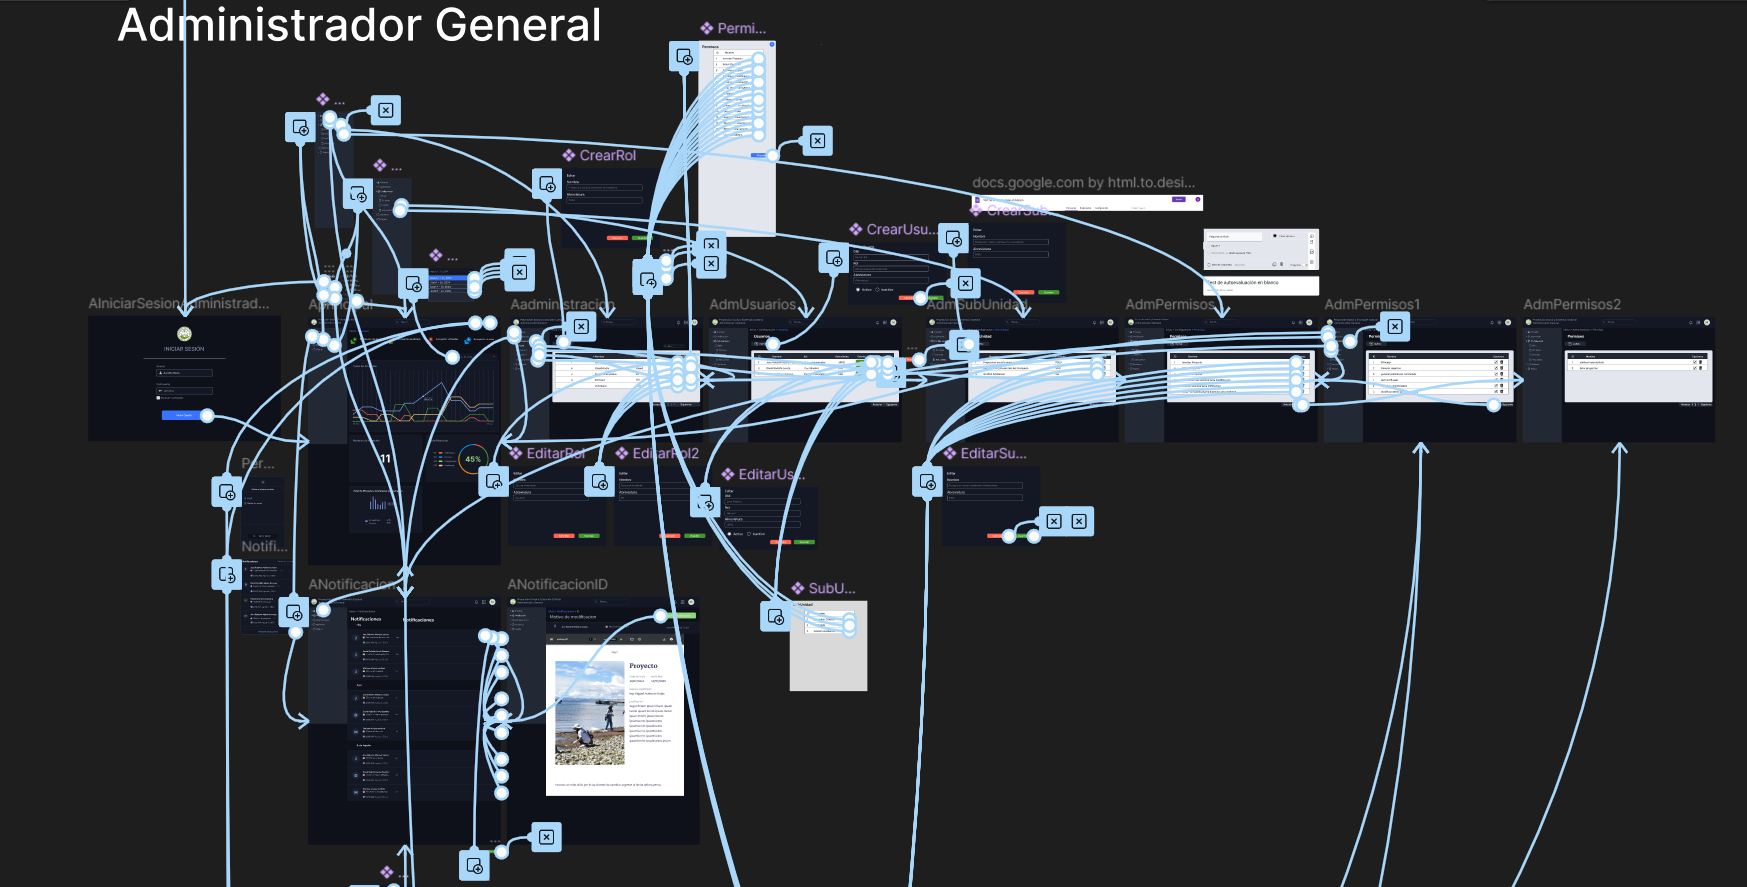
\includegraphics[width=0.8\textwidth]{images/figma_admin_general.png} 
    \label{fig:admin_general} 
\end{figure} 
\FloatBarrier
